%!TEX root = ../report.tex

\begin{document}
    \chapter{Evaluation}
	Below are the results of model compression implementations.
	
	\section{Pruning Methods}
	Methods compared include L1 norm pruning \cite{Li2016PruningFF}, L1 pruning with batch normalization and induced sparsity \cite{Liu_2017_ICCV}, and weight pruning \cite{Han2015DeepCC}. These methods are compared based on the FLOP reductions that it acclaims.
	The network used as a baseline is ResNet-56 with pre-activation. Pre-activation on ResNet is used as it is able to alleviate the problem of vanishing gradients on deeper networks. \cite{10.1007/978-3-319-46493-0_38} 
	\begin{figure}
		\centering
		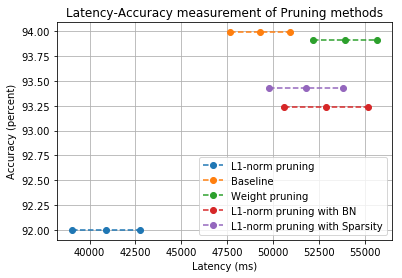
\includegraphics[width=0.7\linewidth]{pruning_result_2}
		\caption{Comparison of Latency for Pruning Methods}
		\label{fig:pruning_result_2}
	\end{figure}
	
	\begin{figure}
		\centering
		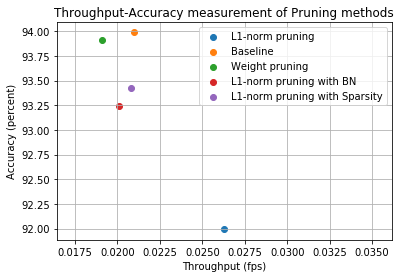
\includegraphics[width=0.7\linewidth]{throughput_2}
		\caption{Comparison of Throughput for Pruning Methods}
		\label{fig:throughput_2}
	\end{figure}
	
	In the figure, the dot in the middle is the measurement, right and left dot is the standard deviation of the measurement.
\end{document}
